\section{Background}
\subsection{Overview of long-short trading strategies}
When someone has a positive expectation for the performance of an asset in the market, the simplest way to profit from it is to buy that asset. If the asset is a stock for example one could buy shares of that stock. If the expectation was correct, when that asset goes up in price, those shares can be sold and the difference in price is kept as profit. Buying an asset is generally called "going long".

But what if one expects a negative performance for some asset? It is also possible to profit from these views by doing the opposite. The share can be borrowed and sold in the market, to be later bought at a lower price and keeping the difference as profit. This is generally called "going short" on an asset.

There are a few reasons why going short on an asset is however not as straightforward as going long. For one, even though the borrowing of shares is a very streamlined process nowadays it is still more cumbersome than simply buying the asset. Furthermore, it entails borrowing costs for the time while the position is open and it is also riskier. While long positions have a maximum loss of 100\% -- when the price of the asset goes to 0 -- short positions can lose more than 100\%. If the price triples for example and one is to close the position, one must buy the asset spending three times the amount of money originally received when selling the borrowed shares, leading to a loss of 200\%. In order to prevent this situation and to make sure that the shares are always given back to the lender, short positions -- like leveraged positions --  can also lead to margin calls, materializing our losses when there are sudden price movements in the market.

Allowing for short positions however also has some benefits. It allows asset managers or traders to profit also from negative views on some assets, not only from positive ones. Taking a portfolio view, by removing the constraint stating that all positions must be positive, the new universe of possible portfolios is much wider. This can be seen very clearly in the asset allocation problem, where by removing the short selling constraint the efficient frontier is expanded and better portfolios can be formed. 

One of the possible formulations for the optimal portfolio allocation problem is the following:

$$
\begin{aligned}
    \text{min} \quad & \sigma_p^2 = \mathbf{w}^\top \Sigma \mathbf{w} \\
    \text{s.t.} \quad & \mathbf{w}^\top \mathbf{r} = \mu \\
    & \mathbf{w}^\top \mathbf{1} = 1 \\
    & \mathbf{w} \geq 0
\end{aligned}
$$


Where $\sigma_p^2$ is the portfolio variance, $w$ is the vector of portfolio weights, $\Sigma$ is the matrix of asset covariances, $r$ is the vector of asset returns and $\mu$ is the target portfolio return. 

The second constraint is the no-leverage constraint, assuming that the portfolio is self-financed, while the third constraint is the no-short-selling constraint, where all portfolio weights are forced to be positive. 
The difference between including and not including the last constraint can be observed in \autoref{fig:efficient-frontier-comparison}, where the portfolio problem has been solved for different target returns for each of the two discussed formulations. 

\begin{figure}[h]
    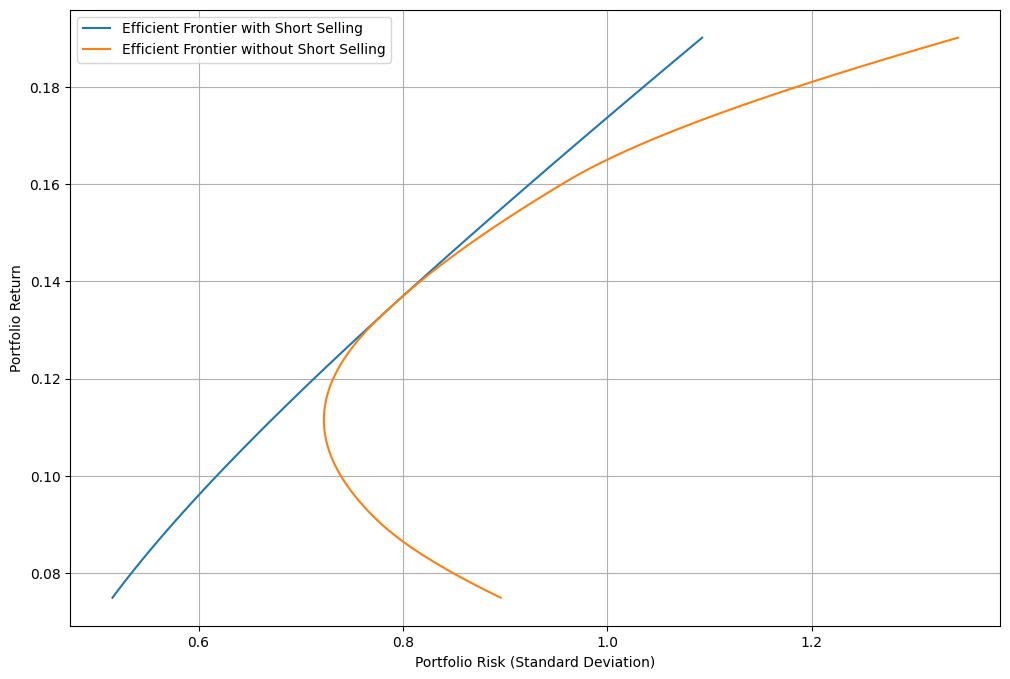
\includegraphics[width=\linewidth]{assets/efficient-frontier-comparison.png}
    \caption{Comparison of efficient frontiers with and without short selling constraint}
    \label{fig:efficient-frontier-comparison}
\end{figure}

As it can be clearly seen, for a given risk level the optimal portfolio without the short selling constraint has expected returns equal or greater than the optimal portfolio with the constraint. 

Any strategy that allows for both the buying and selling of assets is called a long-short trading strategy, and there are many such strategies with different purposes and characteristics. The strategy that will be studied in this work belongs to a type of long-short strategies called pairs-trading strategies.

\subsubsection{Pairs-trading strategies}
These strategies were first developed by a group of traders at Morgan Stanley in 1985 under the leadership of Nunzio Tartaglia (\cite{pole_2011}) and they follow a very simple principle. There are sometimes pairs of assets that move very similarly, like the case of Aveco Biotechnology and Dover Corporation, whose prices are shown in \autoref{fig:cointegrated-assets}.

\begin{figure}[h]
    \captionsetup{justification=centering}
    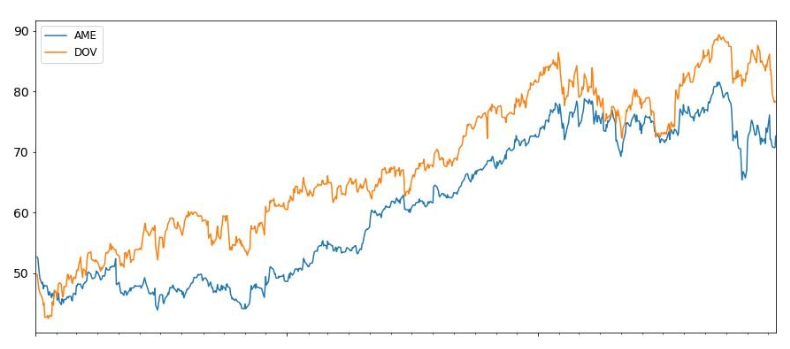
\includegraphics[width=\linewidth]{assets/cointegrated-assets.png}
    \caption{Stock prices of two cointegrated assets. Source: \href{https://hudsonthames.org/definitive-guide-to-pairs-trading/}{Hudson and Thames: The comprehensive introduction to pairs trading}}
    \label{fig:cointegrated-assets}
\end{figure}

If one thinks for some reason that one of the two assets is going to outperform the other, then a long position is entered in that one and a short position is entered in the other one. That way, the general movement of the market can be taken out of the position, and the profit of the trade will only depend on the difference in movement between the two assets, and not on the market movements affecting both assets. 
This can be seen more clearly with a small extension to the $CAPM$ model, where asset specific component for the returns are included.
\begin{equation}
    r_a=r_f+\beta_a(r_M-r_f)+ r_a^s+ \epsilon_a
\end{equation}
\begin{equation}
    r_b=r_f+\beta_b(r_M-r_f)+ r_b^s+ \epsilon_b
\end{equation}

A position can be chosen for both assets with position sizes $\Delta_a$ and $-\Delta_b$ and $\Delta_a\beta_a=\Delta_b\beta_b$ so that
\begin{equation}
    \label{e:market-disappears}
    r_p=\Delta_ar_a-\Delta_br_b=(\Delta_a-\Delta_b)r_f + \Delta_a r_a^s - \Delta_b r_b^s + \epsilon_p
\end{equation}
where $\epsilon_p = \Delta_a \epsilon_a - \Delta_b \epsilon_b$.

As it can be seen in equation \eqref{e:market-disappears}, the market or non specific part of the returns disappears. The portfolio returns end up depending mainly on the specific part of the returns of each of the assets, or more specifically, on the difference between these components. 

Having a strategy with returns independent to the performance of the market can be very attractive, as this strategy can in theory provide positive reutrns regardless of the general market behaviour and trends. Furthermore, by combining several sources of uncorrelated returns -- as none of them are correlated to the market any longer -- one can achieve a very well diversified portfolio with a great risk adjusted performance. 

The question of how one can find two such assets which "move very similarly" requires a bit more consideration. As outlined by \cite{review_statistical_arbitrage} there are many approaches studied in the litereature to finding such pairs. These include the Distance approach, Time series approach, Stochastic control approach, Copula approach, Principal Component Analysis approach, etc. The one that will be relevant here however is one method which relies on the idea of cointegration. 

Suppose there are two time series $X_1, X_2$, with order of integration $d$. That is, by differentiating the time series $d$ times the resulting time series is covariance-stationary -- its mean and autocovariance are constant through time and its variance is finite. The two time series are cointegrated if there exists a linear combination of the two through which the resulting time series has an order of integration of less than $d$. This can also be applied to groups of more than two time series.  

Note that this is similar to the removal of the market returns explained above but even more powerful. If enough cointegrated return time series are found, one could combine them having a portfolio with returns with a constant mean. If we know for a fact that our returns have a constant positive mean, we could have assured profits!

\subsection{Significance of understanding PnL drivers}
The Profit and Loss (PnL) of a trading strategy represents its net financial outcome, capturing the time series of gains or losses from all the trades executed under that strategy. However, the PnL itself is an aggregate measure that obscures the underlying factors contributing to the performance. Understanding the PnL drivers of a trading strategy is crucial for several reasons, particularly when it comes quantitative strategies with like the one studied in this work where the trading decisions cannot be intuitively understood. Identifying and understanding these drivers allows traders, portfolio managers, and risk managers to assess the effectiveness, risks, and potential of the strategy.

\subsubsection{Classes of PnL drivers}
\label{sec:classes-pnl-drivers}
PnL drivers are essentially the components that influence the profitability of a trading strategy. In the context of long-short strategies, these drivers can include:
\begin{itemize}
    \item \textbf{Market Exposure (Beta)}: The extent to which the strategy is exposed to broader market movements. Even in market-neutral strategies like pairs trading, unintentional beta exposure can impact PnL, especially in volatile market conditions. \cite{sharpe_1964}
    \item \textbf{Factor Sensitivities}: These refer to the strategy's exposure to various risk factors such as size, value, momentum, and volatility. For instance, a strategy with significant unintentional exposure to the momentum factor may perform well in trending markets but suffer during mean reverting market periods. \cite{asness_moskowitz_lasse_pedersen_2013}
    \item \textbf{Alpha Generation}: Alpha represents the excess return of the strategy over a benchmark or risk-free rate, and it is often seen as a key driver of PnL in active strategies. Identifying sources of alpha -- whether from market inefficiencies, behavioral biases, or other anomalies -- is central to understanding a strategy's potential for sustainable returns. \cite{feibel_2003}
    \item \textbf{Transaction Costs and Slippage}: These operational factors can erode PnL, particularly in high-frequency trading or strategies with low holding periods. Understanding how transaction costs impact net returns is vital for accurate performance measurement and optimization. \cite{gerhold_guasoni_muhle_2013}
    \item \textbf{Liquidity and Market Impact}: The liquidity of assets in the trading universe and the strategy's own impact on market prices can also be significant PnL drivers. Strategies that depend on trading less liquid instruments may encounter significant market impact, affecting overall profitability. \cite{tarun_chordia_roll_avanidhar_subrahmanyam_2001}.
\end{itemize}

\subsubsection{Importance of understanding PnL drivers}
Understanding each and all of the different drivers of a given strategy has some very relevant advantages:
\begin{itemize}
    \item \textbf{Performance Attribution and Enhancement}: By decomposing PnL into its drivers, traders can pinpoint which elements of their strategy are contributing positively or negatively to performance. This allows for targeted improvements, whether through refining factor exposures, reducing costs, or enhancing alpha generation. \cite{grinold_kahn_1999}
    \item \textbf{Risk Management}: Knowledge of PnL drivers facilitates better risk management by highlighting potential sources of risk that may not be evident from aggregate performance metrics. For example, excessive exposure to a particular risk factor can lead to significant losses if market conditions shift. \cite{ang_2014}
    \item \textbf{Strategic Adjustment and Adaptation}: Markets are dynamic, and the efficacy of a trading strategy can evolve over time. For example, historically value companies have outperfomed growth companies, but in some of the recent years this trend has reversed. A strategy that derived its performance from exposure to this factor would be affected. Understanding the underlying PnL drivers allows traders to adjust their strategies in response to changing market conditions or factor dynamics, thus maintaining or improving performance over time. \cite{lo_2004}
    \item \textbf{Investor Communication and Transparency}: For portfolio managers, clearly articulating the drivers of PnL is essential for building and maintaining investor trust. Investors are increasingly demanding transparency and want to understand the sources of returns and the risks involved in the strategies they are investing in. \cite{elif_baykal_2019}
\end{itemize}
\subsection{Factor models}
The key tool to understanding these key drivers will be factor models. Since the classical asset pricing model proposed by \cite{sharpe_1964} and \cite{lintner_1975}, many academics and practitioners have expanded and relied on factor models to describe and model asset returns. The idea behind them are quite straightforward. There exist a series of factors -- which are external known variables -- which can be used to model the returns of different assets. Each of the assets has different exposures to each of the factors, which lead to the different returns for the different assets. The general formula for factor models is thus
\begin{equation}
    r_k = \alpha_k + \sum_{i}\beta_i^k f_i + \epsilon_k
\end{equation}
where $\beta_i^k$ are the different factor loadings for asset $k$ corresponding to each of the factors $f_i$. 
Note how the classical $CAPM$ model is one such model with only one factor, the excess market returns. 
\begin{equation}
    r_a=r_f+\beta_a(r_M-r_f) + \epsilon_a    
\end{equation}

The same models that work for explaining past returns can also be used for modeling expected returns, when all the factors are stated in expected terms such as
\begin{equation}
    E\left[r_a\right]=r_f+\beta_a(E\left[r_M\right]-r_f)
\end{equation}

Another classical factor model is the one introduced by \cite{french_1992}, where two additional factors are added to compensate for the fact that there is some information regarding stock returns that isn't captured in the exposure to the market excess returns. For example, historically value stocks have outperformed growth stocks while the smaller companies within the S\&P500 have outperformed the bigger ones.
\begin{equation}
    r_a=r_f + \beta_{r_M-r_f}(r_M-r_f) + \beta_{HML}HML + \beta_{SMB}SMB + \epsilon_a
\end{equation}

These factors will be explained in more depth when the factor model used in this work is presented. 

Since the appearence of these two factor models, a huge compendium of different factors have appeared and proven with different levels of success to be determinant to stock returns. It makes no sense to review here all of these factors. However, a brief overview of the differnt types of factors can be seen in \cite{connor_1995}.
\begin{itemize}
    \item \textbf{Macroeconomic factors}: These factors are observable economic time series relating to the general economy. Some examples of such factors are the inflation rate, excess returns of long-term government bonds, percentage change in industrial production, etc. 
    \item \textbf{Fundamental factors}: These factors are characteristics of each of the stocks which have been shown to have predictive power over the returns of said stock. Some examples are firm size, BTM ratio, dividiend yield, etc. 
    \item \textbf{Statistical factors}: These factors use different statistical methods such as Maximum Likelihood Estimation or Principal Component Analysis on cross sections of asset returns to try to extract some underlying factors to all returns. 
\end{itemize}
Even though these may seem like different types of the same thing, in reality there is a crucial difference between Macroeconomic and Statistical factors and Fundamental factors. In the first two, the factors -- common to all stocks -- are observed exogenously, and then the factor loadings are obtained through a time series regression. For Fundamental factors however the process is the opposite. The betas are the ones exogenously derived, while the factor returns have to be obtained from the betas and the asset returns through a cross-sectional regression, as these factor returns cannot be observed anywhere. 
%\subsection{Literature review}
%\textcolor{green}{IS THIS REALLY NECESSARY?}
%Main long-short papers, factor models, factors influencing PnL, identify gaps
% \subsection{Objectives and scope of study}
% Once the basic building blocks of the study have been layed down, it is possible to explain what the purpose of the study is. 

% First, a pairs-trading implementation proposed by \cite{gallego_2023} is reviewed and adapted, from a fundamental point of view to add some changes to the way the strategy proposed by \cite{ioannis_2023} was implemented and from a technical point of view, so it is able to successfully perform a backtest on a much larger universe of assets. Then, this strategy is run on an extended universe of assets and its performance is analyzed by its own merit and in comparison to a benchmark strategy. The performance is then dissected into the long and short positions sepparately and each leg is further analyzed. 
% Then, a primary factor model is implemented and the returns of the strategy are analyzed through this model.  
% Lastly, the alpha obtained by the strategy according to said model is further analyzed through a secondary fundamental factor model in order to further extract all possible key drivers of the returns of the strategy. 

% Out of all the types of PnL drivers outlined in section \nameref{sec:classes-pnl-drivers}, only market exposure, some factor sensitivities and alpha generation are analyzed. Transaction costs are considered negligible due to the daily frequency of transactions and the small impact compared with the other factors, while slippage and liquidity and market impact have also been ignored due to the high trading volume of the selected universe of assets, the S\&P500. 
